\documentclass[aspectratio=169,10pt]{beamer}
\usetheme{default}
\usefonttheme{professionalfonts}
\usepackage{graphicx}
\usepackage{booktabs}
\usepackage{array}
\usepackage{xcolor}
\definecolor{ink}{HTML}{0F172A}
\definecolor{muted}{HTML}{475569}
\definecolor{blue}{HTML}{484878}
\definecolor{red}{HTML}{B64342}
\definecolor{green}{HTML}{166534}
\setbeamercolor{normal text}{fg=ink,bg=white}
\setbeamercolor{frametitle}{fg=ink,bg=white}
\setbeamertemplate{navigation symbols}{}
\setbeamertemplate{footline}{}
\setbeamertemplate{headline}{}
\setlength{\tabcolsep}{4.8pt}

\begin{document}
\begin{frame}[t]{Track B UNRATE: persistence beats richer ML}
\vspace{-0.25em}
{\small\color{muted} 24-month fixed input window $\cdot$ look-ahead $h \in \{1,3,6\}$ months $\cdot$ metric: mean absolute scaled error (MASE)}

\vspace{0.8em}
\begin{columns}[T,totalwidth=\textwidth]
  \begin{column}{0.62\textwidth}
    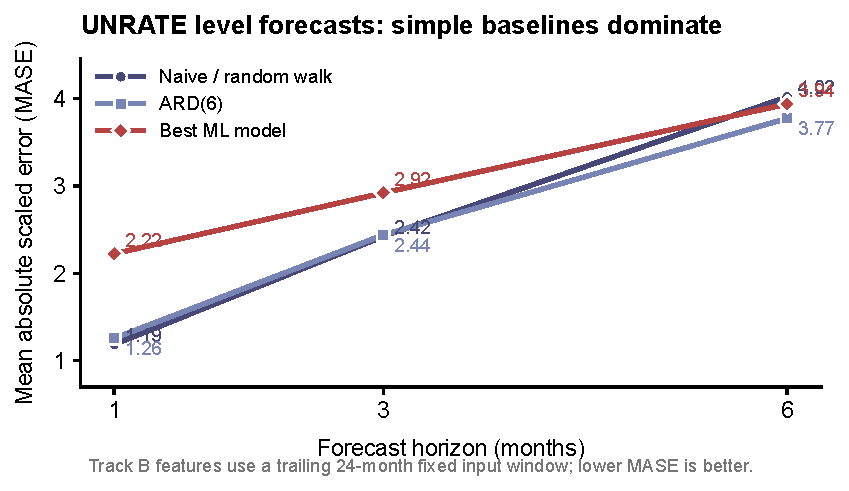
\includegraphics[width=\linewidth]{../figures/track_b_unrate_mase_nature.pdf}
  \end{column}
  \begin{column}{0.35\textwidth}
    \textbf{Best model by horizon}\\[-0.35em]
    {\scriptsize Lower MASE is better. MAE is in percentage points of unemployment.}
    \vspace{0.45em}

    \begin{tabular}{@{}r l r r@{}}
    \toprule
    $h$ & Model & MAE & MASE \\
    \midrule
    1 mo & Naive / Random Walk & 0.153 pp & 1.185 \\
3 mo & Naive / Random Walk & 0.313 pp & 2.424 \\
6 mo & ARD(6) & 0.486 pp & 3.774 \\
    \bottomrule
    \end{tabular}

    \vspace{1.0em}
    \textbf{Interpretation.}\\[-0.2em]
    {\small UNRATE levels are highly persistent. With interpretable Track B inputs, richer ML models do not beat the naive/ARD baselines.}

    \vspace{0.8em}
    {\scriptsize\color{muted} Track B: UNRATE level/delta, building permits, S\&P 500, consumer sentiment, and 10Y--3M yield spread level/delta.}
  \end{column}
\end{columns}

\vfill
{\tiny\color{muted} Source: \texttt{notebooks/03\_track\_b\_unrate\_fixed\_window\_mase.ipynb}; results: \texttt{results/track\_b\_unrate\_24m\_mase\_metrics.csv}.}
\end{frame}
\end{document}
